\documentclass[conference]{IEEEtran}

\usepackage{graphicx}
\usepackage{subfigure}


\hyphenation{op-tical net-works semi-conduc-tor}


\begin{document}
%
% paper title
% can use linebreaks \\ within to get better formatting as desired
\title{Better JavaScript Runtime Understanding by Automated Function Name Extraction}


% author names and affiliations
% use a multiple column layout for up to three different
% affiliations
\author{\IEEEauthorblockN{Salman Mirghasemi}
\IEEEauthorblockA{\'Ecole Polytechnique F\'ed\'erale de Lausanne\\
Lausanne, Switzerland\\
salman.mirghasemi@epfl.ch}
\and
\IEEEauthorblockN{John J. Barton}
\IEEEauthorblockA{IBM Research - Almaden\\
San Jose, USA\\
johnjbarton@johnjbarton.com}
\and
\IEEEauthorblockN{Claude Petitpierre}
\IEEEauthorblockA{\'Ecole Polytechnique F\'ed\'erale de Lausanne\\
Lausanne, Switzerland\\
claude.petitpierre@epfl.ch}}
\maketitle


\begin{abstract}
Understanding JavaScript code due to its dynamic, weakly-typed nature is complicated. Developers usually understand JavaScript programs by running them and examining their elements at runtime. However, understanding concrete values, particularly user-defined and function objects, is not always straightforward. Function names can aid in this regard; they can apear as the constructor name in object representation or as the functions identifier in callstack. Unfortunately, a very low proportion (less than 15\%) of JavaScript functions are named. We propose an approach for automated function naming based on source code analysis. We applied our approach over two relatively large JavaScript programs.
\end{abstract}

\section{Introduction}
The unique and important role of JavaScript in web programming is undeniable. With the wave of ``Web 2.0", JavaScript has become the inevitable part of almost every modern web site. This language is used by 97 out of the web's 100 most popular sites\footnote[1]{http://www.alexa.com}. It is very likely that JavaScript keeps this crucial role at least for the next few years. Along with the growth of demands for more comprehensive user interfaces, the size and the complexity of web applications is increasing. Morover, JavaScript is also becoming a general purpose computing platform with office applications \cite{JSOffice, JSOffice2}, browsers \cite{FAO, GCE} and development environments \cite{Ingalls} being developed in JavaScript \cite{Richards}. There are also proposals for employing JavaScript in server-side applications \cite{SSJSR, CJS}.

To cope with the pace of changes, JavaScript developers need to improve their develoment processes and practices. They need modern editors for writing and editing larger programs and effective tools for understanding complicated JavaScript runtime. However, there has been severe inherent barriers for improving JavaScript tool support. 
Unlike many traditional object oriented languages such as Java and C\#, it does not have classes, and does not encourage encapsulation or even structured programming. JavaScript is a weakly typed language with no type declarations and only run-time checking of calls and field accesses \cite{Richards}. As a direct consequence, the JavaScript code contains less explanatory data about the program elements and their relations. A variable value can be a primitive value, an object with any structure or even a function. One callsite may invoke different function bodies with different number of arities that none of them can be understood from the code. Therefore, the lack of descriptive data in JavaScript code is the most fundumental issue in enhancing JavaScript tool support.

Catching errors early (i.e., before or at the compilation time) is an important feature for development environments. It can save developers' time, prevent bugs and improve the program reliability. However, many errors can not be recognized without a strong typing stystem. To attack this issue a few static typing systems have been proposed for JavaScript \cite{Anderson, Anderson2, Heidegger, Thiemann}. These approaches discover the type of values and object structures for a variable by statically analyzing the source code and possible program control flows lead to the variable assignment. These discovered facts about variable types are not only useful for catching errors but to provide modern editing features such as auto-complete and refactoring in development environments. Moreover, these infered data can help in code coprehension if they are properly presented. Nevertheless, none of the mentioned approaches provided effective means for sharing this information with the developer. 

Developers usually understand JavaScript code by examining the running program in debuggers. At runtime, concrete values are available and developer can directly check and understand object structures and control flows. Understanding a concrete value, particulary for non-primitive values such as objects and functions, is not always straightforward. To facilitate understanding these complex values at the first place, debuggers show a summary of these objects. For example, in case of user-defined objects, the name of object's constructor can be very helpful in the object summary. It can work like a class name and summarizes the object structure.

Functions are central to program comprehension in JavaScript. They are first-class objects that are used for different purposes by developers; 
they may be used as an object  constructor, a clousure scope(module) or even  passed as an argument in a function call. However, there is a subtle issue with JavaScript functions that makes working with them in debuggers quite impossible: functions can be defined and created with no name or identifier. The function name is necessary for referring and recalling the function's functionality, but only a small proportion(less than 15\%) of JavaScript functions are named.

\begin{figure*}[htp]
\centerline{
\subfigure[Firefox Firebug Debugger]{\label{fig_object_first_case}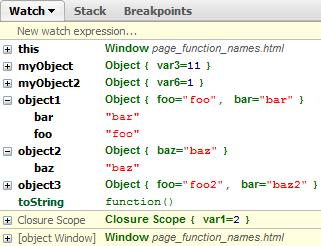
\includegraphics[width=.47\textwidth,height=.27\textheight]{fbug-objects.jpg}}
\hfil
\subfigure[Google Chrome Debugger]{\label{fig_object_second_case}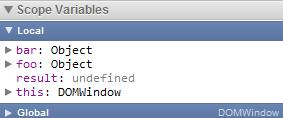
\includegraphics[width=0.47\textwidth,height=.27\textheight]{chrome-objects.jpg}}}
\caption{These two pictures show the variables view of Firebug and Google Chrome JavaScript debuggers paused at the same breakpoint.}
\label{debuggers-objects}
\end{figure*}

In this paper, we propose automated JavaScript function naming based on extracted data by anaylizing the source code. The candidate function names can be used in debuggers for more descriptive object summaries and callstack view. Moreover, these function names can be used in integration with proposed JavaScript typing systems for providing modern editing features in development environments.


\section{The Function Naming Problem}

The importance of function names is not only limited to call stack view. A function can be used as a constructor for constructing new objects. The constructor name like class name in traditional languages such as Java, can be used in object representation. It can assist developers in understanding the structure and role of the object without looking into its properties. 
%function body(source), function object

In JavaScript, defining \textit{identifier} for functions is optional. A function can be assigned to a variable or an object property with any name. Therefore a function object can be called by different names during in life time. 
%___ why it is hard




\subsection{Constructor Name}
Figure~\ref{debuggers-objects} shows the variables view of Firefox and Google Chrome debuggers, paused at the same breakpoint. To know a variable value developer first check the summary value presented besides the variable name. If the summary value is not enough, then developer can expand the variable node to examin variable properties. In this case, the values of all variables are created using a constructor and the constructor name can be included in the summary. However, instead of the name of constructor which can hint the developer about the object structure, only \texttt{Object} is shown. 

%Many developers develop JavaScript in object-oriented way.
%

JavaScript is an imperative, objectoriented
language with Java-like syntax, but unlike Java it employs
a prototype-based object system. An object is a set of properties,
a mutable map from strings to values. A property that evaluates
to a closure and is called using the context of its parent object
plays the role of a method in Java. Each object has prototype field
which refers to another object. Property lookup involves searching
the current object, then its parent, and its parent until the property
is found. The JavaScript object system is extremely flexible. As a
result, it is difficult to constrain the behavior of any given object.
For example, it is possible to modify the contents of any prototype
at any time or to replace a prototype field altogether. In JavaScript,
any function can be a constructor for a �class� of objects, and
contains a prototype field, initially referencing an empty object.
The new keyword creates an object based on the prototype field and
using the function as a constructor. The semantics of new is simple,
but unusual: first, an empty object is created, with its parent set
to the object referenced by the prototype field of the constructor
function; second, the constructor is called, with this bound to
the new object. The object referenced by the keyword this is not
determined by lexical scoping, but instead by the caller; finally the
return value from the constructor (if any) is discarded, and the new
expression evaluates to this.%richards

\subsection{Callstack View}
Figure~\ref{debuggers-callstack} shows the call stack view of Firefox Firebug and Google Chrome JavaScript debuggers, paused at the same breakpoint. The differences between two call stacks, particularly in the first two frames, are due to different implementations of event handling in the underlying platforms. Google chrome shows \texttt{anonymouse} as the identifier for three functions which doesn't give any useful information to the developer. The developer has to locate the function by its source file and line number to recall the function functionality. Although Firebug shows more function names, it is also speechless about one function.



\begin{figure*}[htp]
\centerline{
\subfigure[Firefox Firebug Debugger]{\label{fig_first_case}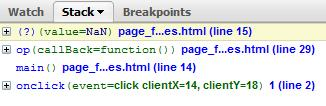
\includegraphics[width=.47\textwidth,height=.15\textheight]{fbug-callstack.jpg}}
\hfil
\subfigure[Google Chrome Debugger]{\label{fig_second_case}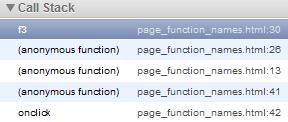
\includegraphics[width=0.47\textwidth,height=.15\textheight]{chrome-callstack.jpg}}}
\caption{These two pictures show the call stack view of Firebug and Google Chrome JavaScript debuggers paused at the same point. 
The Google Chrome debugger is unable to find three function names and The Firebug debugger fails at one case.}
\label{debuggers-callstack}
\end{figure*}


%explain function expression and function declerations
%moreover explain creation of the list of outer scopes.
%Functions can be defined and created with no name or identifier.
In JavaScrip a function can be defined by a function expression or a function decleration \cite{ECMA}. From the same function expression or decleration, function objects are created. In addition to function source code, the clousure scopes are also important for understanding the function operation. The clousure scopes include all available variables to the function at the time of creation. The location of function definition in the source code is enough for knowing the clousure scopes. Therefore, a function body with its location in a source code defines a category of function objects with the similar behaviour.
Is it possible to assing a name to every function object in JavaScript in a way that:
1) Function objects with the same code has the same name.
2) The proposed name recalls the function for the developer.
3) Describes the function behaviour.
%uinque?!
%For example to know an object, developer has to examine the object properties and from the property names and values, some connections
%understanding JavaScript code and its runtime is much harder for developers.
% we propose automatic function naming with these features
% 1) expected by user 2) different situations

\section{Automatic Funcation Naming}
%-- Check here: http://kangax.github.com/nfe/
To choose the most appropriate name for a function which has the characteristics defined in the previous section, we consider two cases. First, assigning a global name to the function which identifies the function in the whole program. Second, naming a function in a call stack.

A function object in JavaScript can be defined by \texttt{function \textit{identifier} (args)\{...\}} or \texttt{new Function(args, source)}.
\subsection{A Global Name for a Function Object}


%\begin{center}
    %\begin{tabular}{ | l | l | l | p{5cm} |}
    %\hline
    %& Type & Sample & Description \\ \hline
    %a & Named & function foo(){...} & The function is named. \\ \hline
    %a & Named & function foo(){...} & The function is named. \\ \hline
    %a & Named & function foo(){...} & The function is named. \\ 
    %\hline
    %\end{tabular}
%\end{center}


\begin{figure}[htp]
\begin{verbatim}
(a) Case 1:
 function foo(){ ... }

(b) Case 2:
 var foo = function { ... } 
 
(c) Case 3:
 var foo = {
     bar : function { ...}
 }

(d) Case 4:

 var foo = function(){
           ....
           return function(){ ... }
 }()
 
(e) Case 5:
 var foo = function(){ 
 					 return ...;
 }()					
 
(f) Case 6:
 var foo = function(){
 
 }()();
 
(g)
 foo(function(){ ... });
 
(h)
 array = [...., function(){},...]
 
(i)
 array[i] = function(){};   

(j)
 eval(); & new Function("");
 
\end{verbatim}
\caption{Different cases of function object creation.}
\label{fig:functionCreation}
\end{figure}

\subsection{Naming Functions in Call Stack}
%new Function ([arg1[, arg2[, ... argN]],] functionBody)
%this[ optall.queue === false ? "each" : "queue" ](function() {})


\begin{figure}[htp]
\begin{verbatim}
(a)
 foo();
(b)
 foo.bar();
(c)
 foo.apply(bar, args);

\end{verbatim}
\caption{Different cases of function object creation.}
\label{fig:functionCall}
\end{figure}

\section{evaluation}
%Firebug, JQuery,

%JQuery
% core.js 


\section{Related Work}
%Another strand of research has tried to investigate how to provide better tools for developers for catching errors early. Being a weakly typed language with no type declarations and only run-time checking of calls and field accesses, it is natural to try to provide a static type system for JavaScript [2, 1, 3, 24, 13]. Finally, after many years of neglect, modern implementations of JavaScript have started to appear which use state of the art just-in-time compilation techniques [10].

%For JavaScript, Anderson et al. proposed a type system with definite and potential types [2, 1, 3], while Heidegger and Thiemann following up on some of their earlier work [24, 18] propose recency types in [13], and Furr et al. proposed a related system for DRuby [9]. While all of these type systems acknowledge some minor simplifications to the target language, they rely on fairly similar assumptions. For instance, Thiemann writes: �Usually, no further properties are defined after the initialization and the type of the properties rarely changes.� This suggests that object types are stable at run-time and can be described using, e.g., traditional rowtypes. In fact all the proposals take the view that an object�s type should be the sum of all possible fields and methods that it could contain, with some of them being undefined; they differ mostly on how to perform strong updates to avoid polluting all properties with undefined values. Interestingly, language implementors make similar assumptions. For instance, Google�s V8 JavaScript engine is reported to optimistically associate �classes� to objects on the assumption that their shape will not change too much, though with a fallback case for highly dynamic objects 3. This design is similar to implementations of one of JavaScript�s influences, Self [5], and is expected to work for the same reasons. As the above mentioned hypothesis is crucial for the applicability and usefulness of the results, it deserves careful study. In fact, we have found a number of similar assumptions in the literature which we list below.We first review the salient features of the language to provide sufficient background for readers unfamiliar with JavaScript.

\section{Conclusion}
In this paper we presented an approach for naming JavaScript functions both
as individual objects and in call stack. 


\begin{thebibliography}{10}

\bibitem{Anderson}
C. Anderson, P. Giannini, and S. Drossopoulou. \newblock Towards Type Inference for JavaScript.
\newblock In \emph{Proceedings of the 19th European conference on Object-Oriented Programming(ECOOP)},
July, 2005.

\bibitem{Anderson2}
C. Anderson and P. Giannini. \newblock Type checking for javascript.
\newblock \emph{Electr. Notes Theor. Comput. Sci.}, 138(2), 2005. 

\bibitem{CJS}
Common JS.
\newblock http://www.commonjs.org/

\bibitem{ECMA}
ECMA International.
\newblock \emph{ECMA-262: ECMAScript Language Specification},
ECMA (European Association for Standardizing Information
and Communication Systems), Geneva, Switzerland, third edition,
December 1999. 

\bibitem{FAO}
Firefox Add-ons.
\newblock https://addons.mozilla.org/en-US/developers/docs/gett ing-started.

\bibitem{GCE}
Google Chrome Extensions.
\newblock http://code.google.com/chrome/extensions.

\bibitem{Heidegger}
P. Heidegger and P. Thiemann.\newblock Recency types for dynamically-typed, object-based languages.
\newblock In \emph{Proceedings of Foundations of Object Oriented Languages (FOOL)},
2009.

\bibitem{Ingalls}
D. Ingalls, K. Palacz, S. Uhler and A. Taivalsaari.\newblock The lively kernel a self-supporting system on
a web page.
\newblock In \emph{Self-Sustaining Systems},
2008.

\bibitem{JSOffice}
JScript development in Microsoft Office 11.
\newblock http://msdn.microsoft.com/ en-us/library/aa202668(office.11).aspx

\bibitem{JSOffice2}
JavaScript development in OpenOffice.
\newblock http://framework.openoffice.org/ scripting/release-0.2/javascript-devguide.html

\bibitem{Richards}
G. Richards, S. Lebresne, B. Burg and J. Vitek.\newblock An analysis of the dynamic behavior of JavaScript programs.
\newblock In \emph{Proceedings of the 2010 ACM SIGPLAN conference on Programming language design and implementation(PLDI)},
June, 2010.

\bibitem{SSJSR}
Server-Side JavaScript Reference v1.2.
\newblock http://research.nihonsoft.org/ javascript/ServerReferenceJS12.

\bibitem{Thiemann}
P. Thiemann.\newblock Towards a type system for analyzing JavaScript programs.
\newblock In \emph{Proceedings of European Symposium on Programming (ESOP)},
2005.

 
\end{thebibliography}



% that's all folks
\end{document}


